        \documentclass{standalone}
        \usepackage{tikz}
        \usetikzlibrary{arrows}
        \usepackage{amsmath}
        \usepackage{amsfonts}
        \begin{document}
        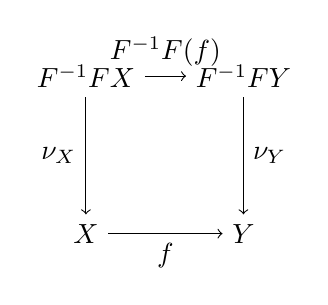
\begin{tikzpicture}

    \node at (0,0) (FFX) {$F^{-1}FX$};
    \node at (2,0) (FFY) {$F^{-1}FY$};
    \node at (2,-2) (Y) {$Y$};
    \node at (0,-2) (X) {$X$};
    \draw[->] (FFX) -- node[above] {$F^{-1}F(f)$} (FFY);
    \draw[->] (FFY) -- node[right] {$\nu_Y$} (Y);
    \draw[->] (X) -- node[below] {$f$} (Y);
    \draw[->] (FFX) -- node[left] {$\nu_X$} (X);
        \end{tikzpicture}
        \end{document}
